\section{Regeln}
\label{sec:Regeln}

\subsection{Regelbeschreibung}
Da in fast allen Fällen ein sehr nah gelegenes Polygon gemeint ist, wird zunächst auf den Abstand aller vorhandenen Polygone etwas aufaddiert,
um den Abstand 0 zu vermeiden, und diese danach nach unseren Regeln zu gewichten um anschließend das Polygon auszuwählen,
welches nach der Gewichtung den kürzesten Abstand hat.



\subsection{Formale Beschreibung}
Sei $ID$ die die Bezeichnung eines Bildes.\\
Sei $t$ ein Tag $(key \to value)$ aus OpenStreetMap.\\
Sei $r(t)$ eine Regel $t \to [0..2]$ \\
Sei $Z_{X}$ die Menge der Tag $t$ für die Gilt: $t$ kommt in X vor. \\
Sei $V$ eine Menge von Verboten $v$.\\
Sei $V_{ID}$ die Menge der Verbote für die gilt: $v$ wird auf dem Bild zu $ID$ abgebildet.\\
Sei $R_V$ eine Menge von Funktionen $r$ für die Verbote $V$\\
Sei $C_{ID}$ die Geocoordinate, an welcher das Bild zu $ID$ aufgenommen wurde. \\
Sei $D_{X,ID}$ der Abstand eines Polygons $X$ zu $C_{ID}$ \\
Sei $O_{ID}$ eine Menge von Polygonen aus OpenStreetMap in der Umgebung zu $C_{ID}$\\
Sei $A_{X}$ die Fläche des Polygons $X$\\
Sei $s(V) : v \to r(t)$  Eine Abbildung von Verbote zu einer Menge von Regeln\\
Sei $P_{ID}$ das gegebene Lösungspolygon zu $ID$.\\
Sei $I(X,Y)$ das Schnittpolygon der Polygone X und Y\\
Sei $o$ ein Offset $\in \mathbb{R}$
\\
Sollte es für ein $t$ kein $r(t)$ geben, so wird die Standartregel:
$r(t) = 1$ angewendet.

\begin{equation}
Gew(ID,X) := (D_{X,ID} + o) * \prod_{r \in s(V_{ID})} \prod_{t \in Z_{ID}} r(t);
\end{equation}

\begin{align}
G(ID) := \{X \in O_{ID} | & Gew(ID,X) < Gew(ID,Y)\\
& \lor \Big(Gew(ID,X)=Gew(ID,Y) \land A_X < A_Y\Big) \forall Y \in O_{ID}\} \notag
\end{align}

\subsection{Beispiel}
Eine Regel kann z.B. so aussehen:\\
Für das Verbot Nichtrauchen: wenn ein Tag den Key 'building' enhält dann halbiere den Abstand. \\
$R_{nichtrauchen} = [r('building') = 0.5]$\\
\newline
Sei der Offset als 1 angenommen und in der Umgebung zu $ID$ nur zwei
Flächen A,B in OpenStreetMap vorhanden.
\begin{itemize}
\item A enthält die Tags: 'building -> yes', 'addr:housenumber -> 34' und hat den Abstand 0.2;
\item B enthält die Tags: 'landuse->residential' und hat den Abstand 0;
\end{itemize}
Daraus errechnet sich:
\begin{itemize}
\item $Gew(ID,A) = (0.2 + 1) * 0.5 * 1 = 0.6$
\item $Gew(ID,B) = (0.0 + 1) * 1 = 1$
\end{itemize}

$G(ID) = A$

\subsection{Maschinelle Überprüfung der Regelsätze}
Um die Güte der verschiedenen Regeln zu überprüfen wird ein Programm geschrieben, welche für jede Regel die die Schnittpolygone von unseren Polygonen mit
den Musterlösungen bildet und anschließen durch je die Fläche unseres Polygons, sowie des Musterlösungspolygons teilt.
Von beiden Zahlen wird das Minimun genommen und als Indicator der Lösungsgüte angesehen.\\
\begin{equation}
f(v,R) := \sum_{q\in S_v} min(\frac{I(P_q,G(q,R))}{P_q},\frac{I(P_q,G(q,R))}{G(q,R)})
\end{equation}
Um die Güte des Regelsatzes für ein einzelnes Verbot vergleichbar zu anderen Verboten zu machen wird abschließend der Indicator durch
die Anzahl der $ID$s welches es beeinflussen geteilt.\\
\begin{equation}
\label{eq:guete}
G"ute(R) := \sum_{v \in V} \frac{ f(v,R)}{\#S_v}
\end{equation}

Wir suchen also einen Regelsatz $R$ für den $G"ute(R)$ maximal ist.


\subsection{Visuelle Überprüfung}
\label{sec:visuelle_ueberpruefung}
\begin{figure}
\centering
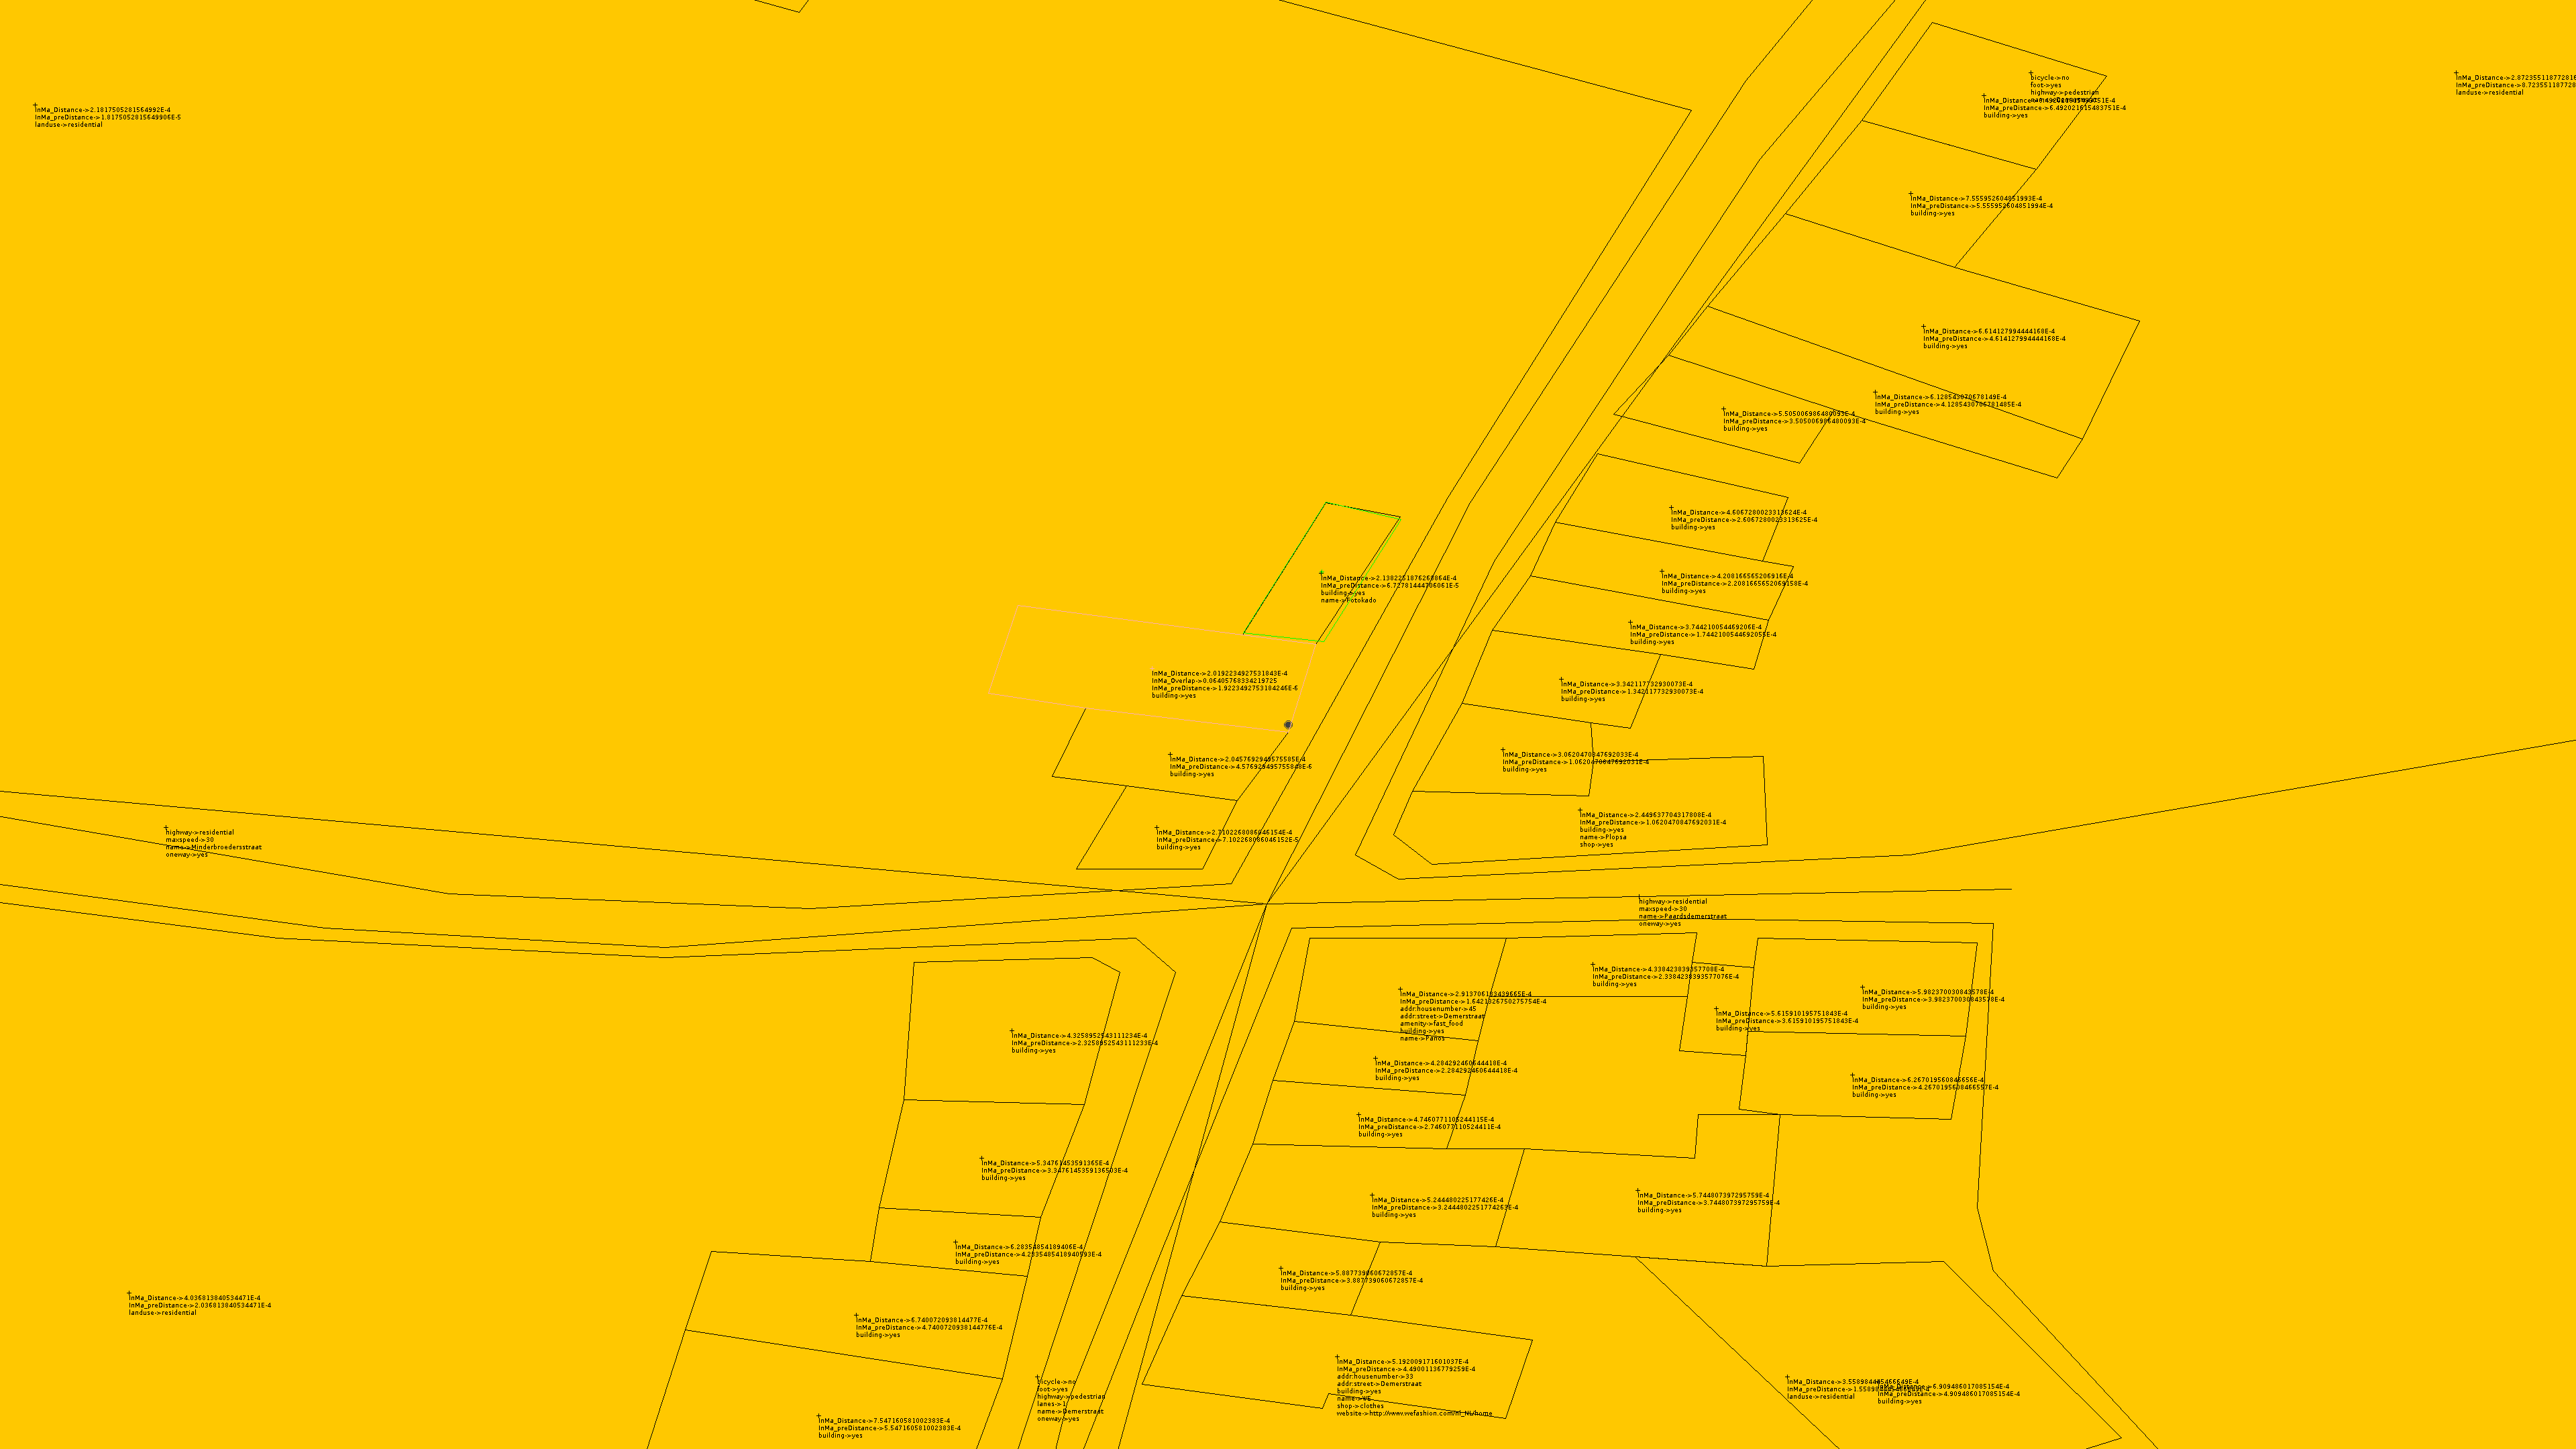
\includegraphics[width=0.8\textwidth]{DataDrawer.png}
\caption{Beispielhafte Ausgabe für Nummer 27}
\label{fig:DataDrawerOrginal}
\end{figure}
Um die KML-Dateien nicht immer manuell in Google-Earth laden zu müssen, wurde eine weitere Klasse geschrieben, welche zur Visualisierung der Daten gedacht ist.
Dabei werden Bilder erstellt, in welchen die Daten aus OSM als schwarze Linien, bzw Polygone eingezeichnet werden. Zusätzlich werden die Tags,
welche die Objekte enthalten zu jedem Objekt eingezeichnet um schnell eine Übersicht zu haben, was wozu gehört.
Um die Güte des Regeldatensatzes, bzw des Algorithmus subjektiv beurteilen zu können, werden die truth, bzw. die von unserem Algorithmus erdachten Polygone
farblich eingezeichnet. So ist eine schnelle Beurteilung, ob man das richtige Poylgon gewählt hat, bzw welche Tags man evtl. noch beachten sollte, möglich.

In \fref{fig:DataDrawerOrginal} ist beispielhaft eine Ausgabe gezeigt. Das Bild hat eine Größe von mehreren Megapixeln, da es sonst zu Überlappungen der Tags kommen
würde wenn man sie größer schreibt. Auch wenn man jetzt noch reinzoomen muss um diese zu lesen, so ist es doch wesentlich bequemer,
als die Überprüfung anhand der OpenStreetMap XML-Dateien. Wie in \fref{fig:DataDrawerZoom} zu erkennen ist, ist das Lösungspolygon in Grün,
das Ergebnispolygon unseres Algorithmus in Pink und die Geocoordinate als schwarzer Punkt eingezeichnet.

Als weiterer Hinweis wird zusätzlich zu jedem Polygon die reale und die gewichtete Distanz zur Geocoordinate, an welcher das Bild gemacht wurde, angegeben.

\begin{figure}
 \centering
 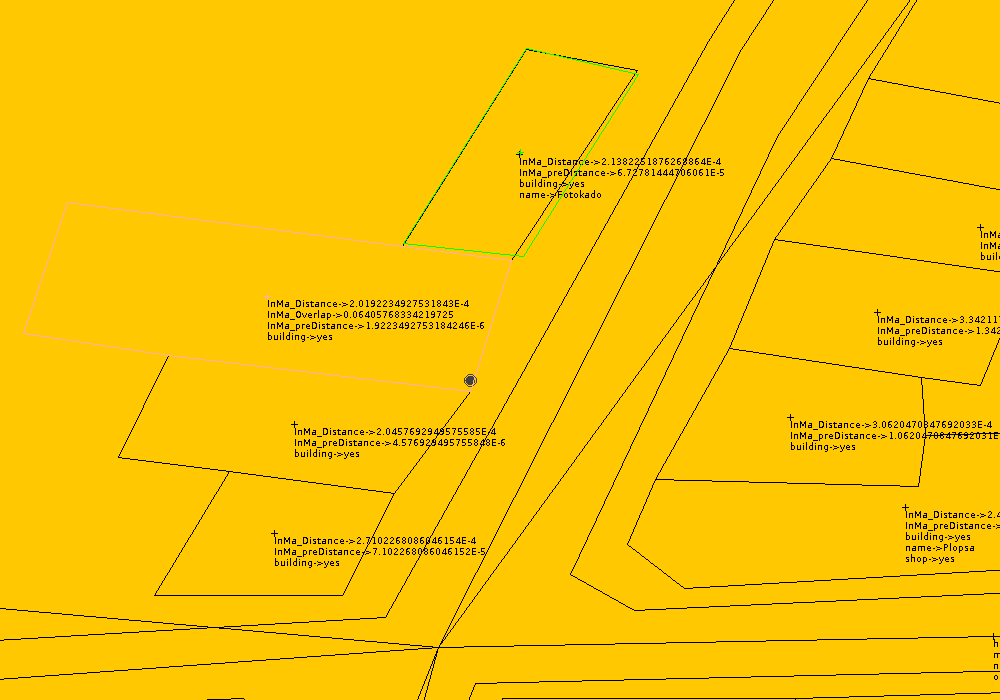
\includegraphics[width=0.8\textwidth]{DataDrawerZoom.png}
 \caption{Reingezoomte Ausgabe für Nummer 27}
 \label{fig:DataDrawerZoom}
\end{figure}

\subsection{Incrementelle Regelerstellung}
Aus dem Testdatensatz werden zunächst alle Datensätze herausgefiltert, welche nicht einfach lösbar sind.
(Vgl. \fref{sec:Testdatensatz})
Es wird mit einem leeren Regelsatz angefangen und dieser anschließend inkrementel erweitert. Dazu wird wie folgt vorgegangen:
\begin{enumerate}
\itemsep-2pt
\item Definiere für jeden Datensatz ein optimales Polygon, bzw einen Overlap-Wert, welcher erreicht werden muss.
\item Der Regelsatz wird auf alle Testdatensätze angewendet. \label{start_inc_alg}
\item Für jeden Datensatz, bei welchem die Regeln nicht das optimale Polygon finden, wird ein Bild wie in \fref{sec:visuelle_ueberpruefung} erstellt. \label{Inc_Image}
\item Dem Benutzer werden alle Bilder, angezeigt und dieser kann nun weitere Regeln hinzufügen oder bestehende ändern.
\item gehe zu \ref{start_inc_alg}
\end{enumerate}

Nach dem Abdecken der einfachen Fälle kann mit den schwierigeren genauso vorgegangen werden.

\subsubsection{Beispiel 1}
Nachdem der Algorithmus mit einem leerem Regelsatz durchgelaufen ist zeigt
\fref{fig:DataDrawerZoom} einen Ausschnitt des Bildes, wie es in Schritt \ref{Inc_Image} erstellt wurde. Wir können nun einfach sehen,
dass es offensichtlich nicht das richtige Polygon ist. Der einzige Unterschied der bestmöglichen Lösung im Vergleich zu dem nächstbesten Polygon ist,
dass das Lösungspolygon noch den Namen Fotokado hat. Desweiteren sehen wir, dass kein weiteres Polygon in der Nähe einen Namen hat.
Fotokado an sich ist jetzt etwas, dass man verwenden könnte, sinnvoller ist es aber, generell zu sagen, dass wenn Namen vorkommen, diese Gebäude
bevorzugt werden sollen. Für Nr. 27 gilt nur: parking="no". Es ist also wahrscheinlich sinnvoll, folgende Regel zu erstellen\footnote{0.8 ist willkürlich gewählt.
0.0 oder 0.5 würden für genau dieses Datensatz auch zum richtigen Ergebnis führen, können aber wiederrum bei anderen ID's hinderlich sein,
da sie eine wesentlich größere Veränderung bewirken.}:
\begin{equation*}
R_{parking=''no''} = [r('name') = 0.8]
\end{equation*}

\subsubsection{Beispiel 2}
\begin{figure}
 \centering
 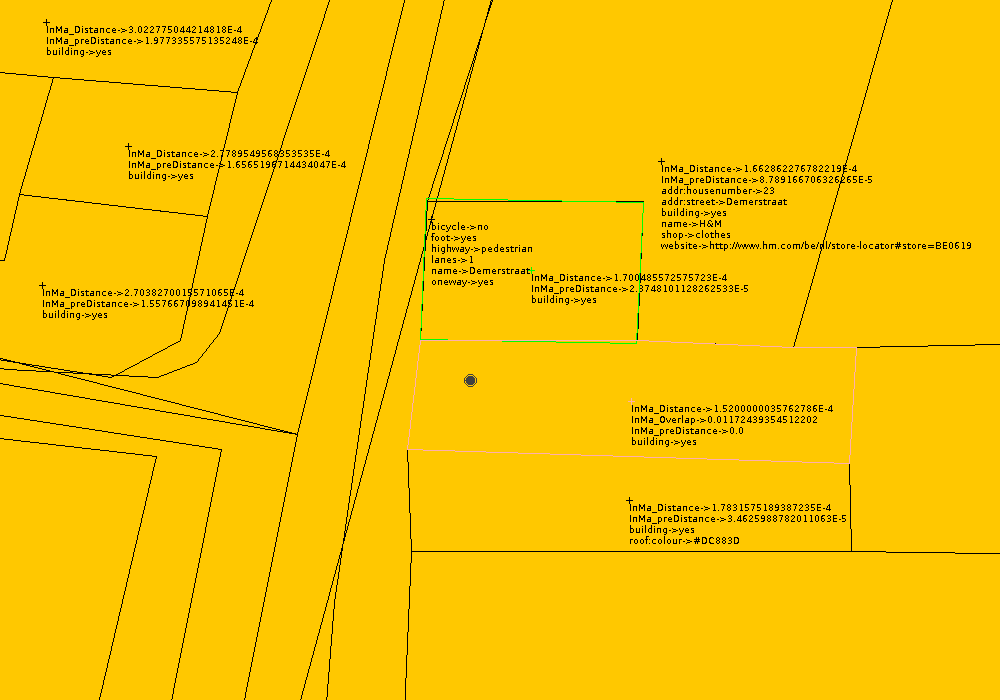
\includegraphics[width=0.8\textwidth]{DataFailZoom.png}
 \caption{Reingezoomte Ausgabe für Nummer 31}
 \label{fig:DataFailZoom}
\end{figure}
In \fref{fig:DataFailZoom} ist zu erkennen, dass es keinen Unterschied bei den Tags für das richtige und das nächstgelegene Polygon gibt.
Hier kann man nicht mehr viel machen und wird wahrscheinlich immer das falsche Polygon ausgeben.


\subsection{Erweiterung}
Um den Fall abzudecken, in welchem in OpenStreetMap keine ausreichenden Daten vorhanden sind, wird um den Punkt $C_{ID}$ ein
Achteck\footnote{Relativ geringer Rechenaufwand bei gleichzeitig bester Annäherung an einen Kreis.} mit Radius $b$ gelegt
und dieses mit der gewichtet nächsten Großfläche geschnitten.
Eine Großfläche X definiert sich dadurch, dass ihre Fläche $A_X$ einen schwellwert $u$ überschreitet.
Es ist zu prüfen ob es sinnvoll ist dieses generell zu tun oder für bestimmte Regel ausser Kraft zu setzen wie
z.B. ein Verbot nach offenem Feuer, welches in einem ganzen Parkgebiet gelten wird.
